\section{Additional thoughts}
\textbf{1. }\textit{Can you think of a case where two
utterances have noticeable differences to a human listener, and may
come with different interpretations or connotations, but still have very
similar MFCCs?}\\

To answer this question first of all we should ask ourselves which features of the speech signal are considered/removed by the MFCCs.\\
First we do a Cepstral analysis, which captures the spectral envelope of the signal, connecting all the formants \footnote{A formant is a region of the frequency spectrum where there is a local/absolute maxima.} of the signal. By doing so we can say that the pitch is being discard. \\Consider for example a voiced phenomena: if you were to analyse the spectrum of the sound \textit{ah} with different pitches you would still see the same envelope though the fundamental frequency changes. This reasoning does not make sense for unvoiced sounds since it is more noisy and there is no harmonic structure, though the spectral envelope exists also for unvoiced sounds. \\ Then we apply a bank of filters to approximate the human perception: humans concentrates on certain regions of the spectral envelope.\\ \\
The main point is that by discarding pitch we are mainly losing information for \textit{voiced phenomena}. Consider again the sound \textit{ah}, it can be used with different meanings based on the pitch: screaming, surprise, etc... though the envelope is still the same. So the MFFCs does not capture this information and a pattern recognition system may fail to recognise the correct situation (surprise, anger,...). \\ \\
Despite that, this method is well suited for those scenarios where the system needs only to recognise the letters and not whether the person is angry or happy. For example, if you want to call someone and you do not want to digit the numbers you can spell all the numbers and the MFCCs feature extraction still would work since we don't care about the pitch in this case.
\\ \\
\textbf{2. }\textit{What about the opposite situation: are there two signals
that sound very similar to humans, but have substantially different
MFCCs?}\\

Signals that are noisy to humans may have a pattern if analysed with frequency/cepstral analysis. For example, consider the sound produced by a fly and an audio sample of the vuvuzelas sound: they sound almost identical to humans, but the spectral envelope is different. Vuvuzela have high constant spectrum at low and high frequencies, and low constant spectrum at medium frequencies, whilst flies produce a sound which is similar to random noise and is flat up to high frequencies. Check figure \ref{fig:fly_vuvuzela} for the frequency and cepstral plots.
\pagebreak
\begin{figure}[h]
\centering
\begin{minipage}{.5\textwidth}
  \centering
  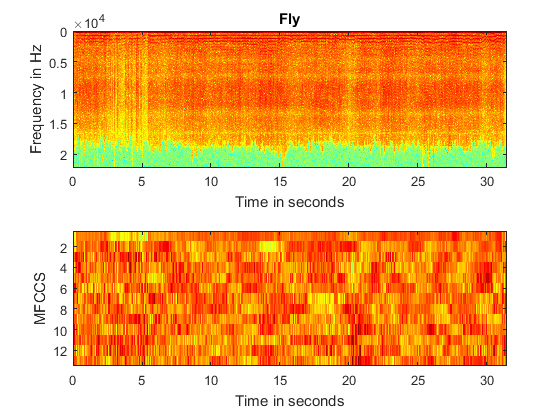
\includegraphics[width=1\linewidth]{./images/fly.png}
\end{minipage}%
\begin{minipage}{.5\textwidth}
  \centering
  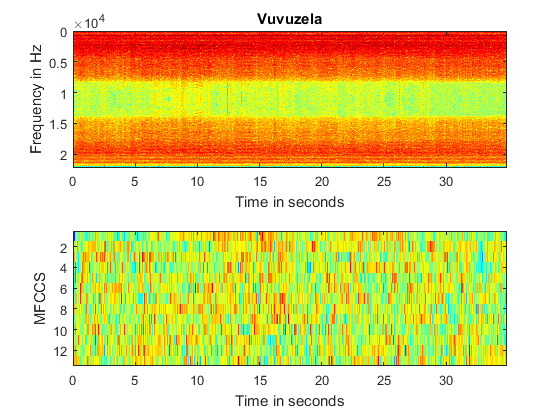
\includegraphics[width=1\linewidth]{./images/vuvuzela.png}
\end{minipage}
 \caption{Spectrogram and Cepstral analysis of the fly (left) and vuvuzelas (right plot) signals.}
 \label{fig:fly_vuvuzela}	
\end{figure}
